\begin{tikzpicture}[remember picture,overlay, inner sep=0pt]
  % Make the tikz bounding box exactly the page
  % \begin{pgfonlayer}{background}
    \path[use as bounding box, fill=black] (current page.south west)
      rectangle (current page.north east);
    \node (LimbImage) [anchor=south west] at (current page.south west) {%
      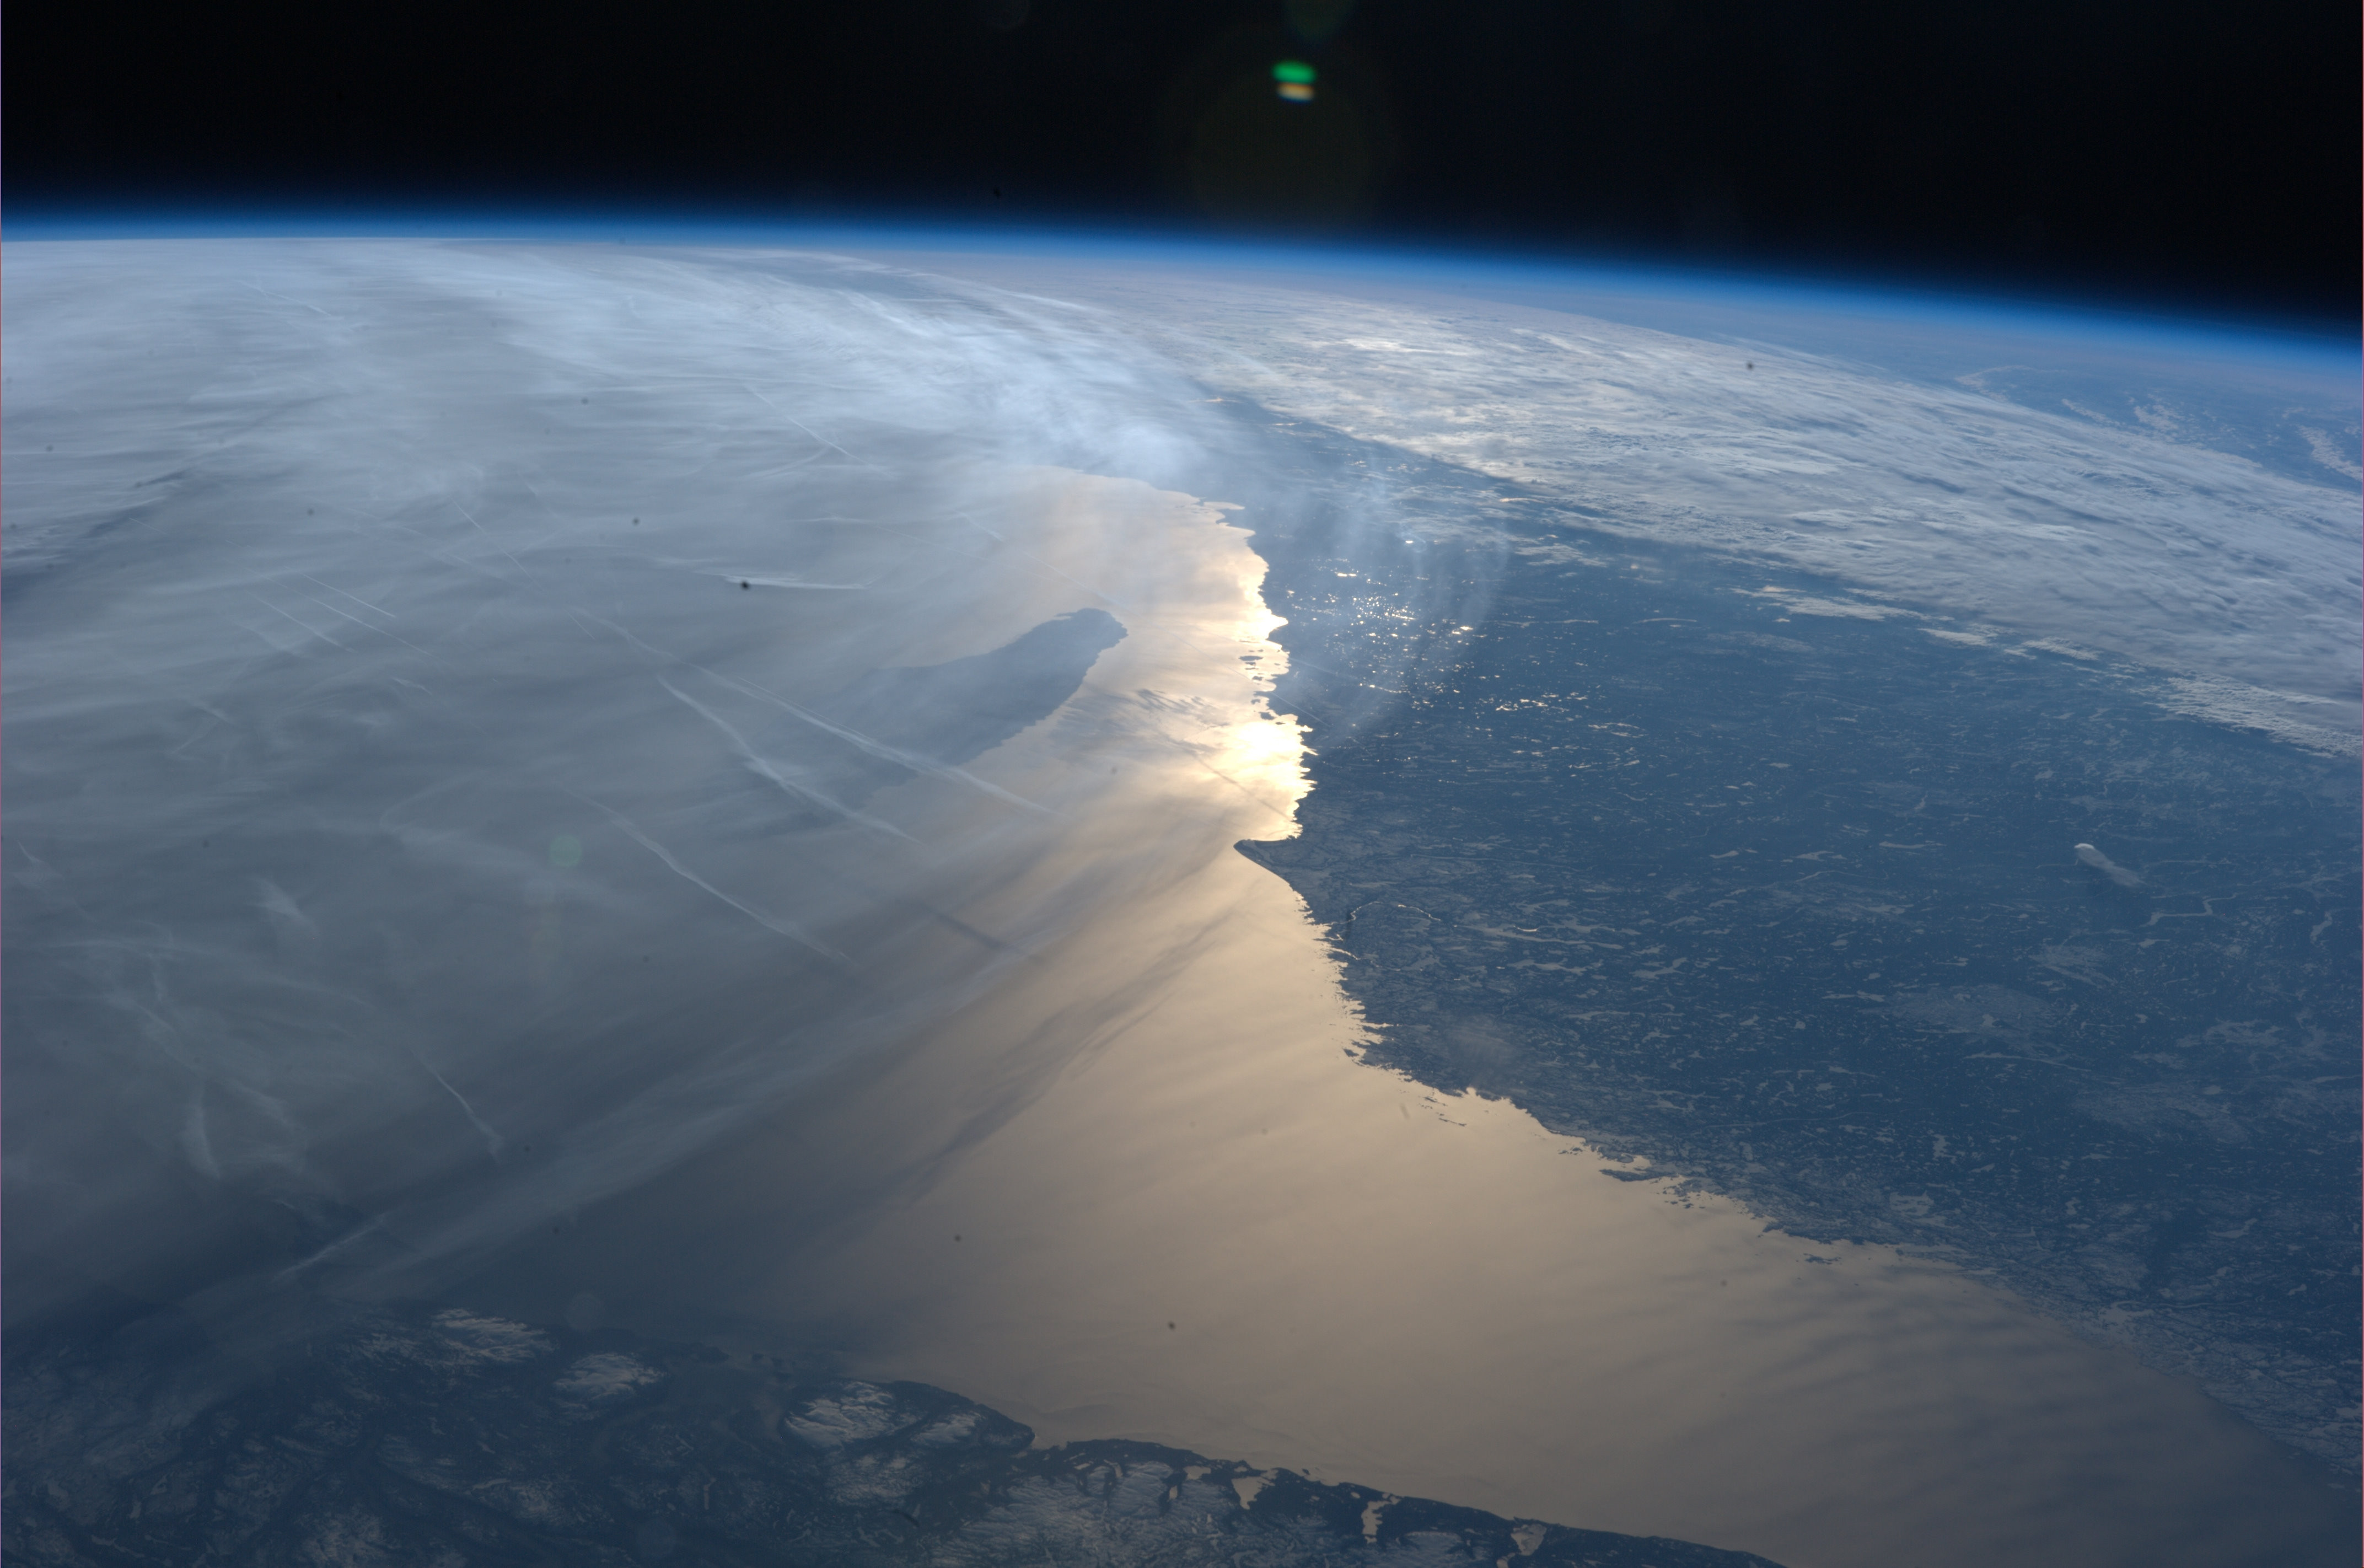
\includegraphics[width=\pagewidth, clip=True, trim=0mm 380mm 0mm 90mm]{figures/iss-limb.jpg}};
  % \end{pgfonlayer}
  %
  \node (NASALogo) [anchor=north east, xshift=-0.4in, yshift=-0.4in] at (current page.north east) 
  {
\includegraphics[width=1.0in]{figures/nasa-meatball.pdf}};
  \node (PreTitle) [anchor=north west, xshift=1.2in, yshift=-0.8in, text width=6.5in, font=\sffamily\fontsize{20pt}{26pt}\selectfont, white] at (current page.north west)
    {Earth Observing System (EOS)\\Aura Microwave Limb Sounder (MLS)};
  \node (MainTitle) [anchor=north west, yshift=-0.5in, font=\sffamily\bfseries\fontsize{32pt}{40pt}\selectfont, white, text width=6.5in, align=flush left] at (PreTitle.south west) {\makeatletter\@title\makeatother};
  \node (Aura) at ($ (current page.south west) + (1.5in, 3.5in) $) {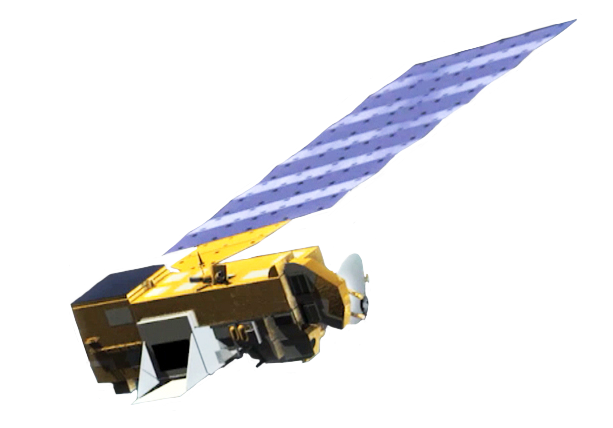
\includegraphics[width=2in]{figures/Aura-Image.png}};
  \draw [ultra thick, orange] ($ (Aura.east) - (0.80in, 0.25in) $) -- ($ (current page.south east) + (0, 2.3in) $);
\end{tikzpicture}\RenderNavBar
